\section{Solution}\label{sec:solution}

In this part, we present our preliminary solution for achieving fast deadlock-free routing reconfiguration.

\subsection{Problem Formulation}\label{subsec:formulation}

\begin{table}
\begin{tabularx}{0.48\textwidth}{ |c||X| } 
	\hline
	$G(V,E)$ & The DCN, where $V$ is the set of all nodes and $E$ is the set of all links. \\ 
	\hline
	$C$ & $C \subsetneq G(V,E)$ is a cycle in $G(V,E)$. \\ 
	\hline
	$P_s$ & The set of paths in the old configuration. \\
	\hline
	$P_t$ & The set of paths in the new configuration. \\
	\hline
	$R_s$ & The set of rules corresponding to $P_s$. \\
	\hline
	$R_t$ & The set of rules corresponding to $P_t$. \\
	\hline
%	$V_p$ & The set of nodes on path p. \\
%	\hline
%	$E_p$ & The set of links on path p. \\
%	\hline
	$R_p$ & The set of rules corresponding to path p. \\
	\hline

	$G_c(V_c,E_c)$ & A configuration dependency graph, where $V_c$ is a set of configuration operations, and $E_c$ is a set of order constraints.\\
	\hline
	$P_c$ & The set of configuration paths in $G_c$\\
	\hline
	$t_o$ & The time to finish an operation $ o \in V_c$.\\
	\hline
	$t(P, G_c)$&The time to configure all paths in $P$ obeying the contrsints in $G_c$.\\
	\hline
	$ts(G_c)$ & A topological sorting of $G_c$, which is a list of configuration operations. \\ 
	\hline
	$TS(G_c)$ & The set of all possible $ts(G_c)$. \\
	\hline
	$P^{(i)}(ts)$& The set of active paths after finishing first i-th operations in $ts(G_c)$.\\
	\hline
%	$P_s^{(i)}(ts)$& The set of remaining paths in $P_s$ after finishing first i-th operations in $ts(G_c)$.\\
%	\hline
%	$P_t^{(i)}(ts)$& The set of activated paths in $P_t$ after finishing first i-th operations in $ts(G_c)$.\\
%	\hline
	$d_{l1,l2}^P$ & The buffer dependency from link l1 to link l2 introduced by the paths in $P$.\\
	\hline
	$P^d_{l1,l2}$ & The set of all paths in $P$ related to  $d_{l1,l2}^P$.\\
	\hline
\end{tabularx}
\caption{The key notations used in the problem formulation.}\label{table:formulation}
\end{table}


\begin{figure}[t]
	\centering
		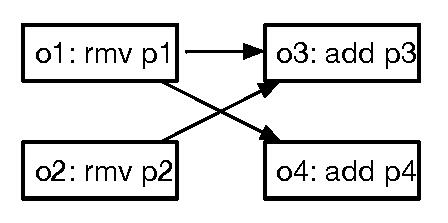
\includegraphics[width=0.45\textwidth] {figs/formulation_example}
	\caption{An example of configuration dependency graph.}\label{fig:cdgraph}
	
\end{figure}

In Table~\ref{table:formulation}, we list the key notations used in our problem formulation. $G(V,E)$ is the DCN. $C$ is a cycle in $G(V,E)$.  $P_s$ is the set of old routing paths, while $P_t$ is the set of new routing paths. $R_s$ and $R_t$ are the set of rules corresponding to the paths in $P_s$ and $P_t$, respectively.  $R_p$ is the set of rules for path p. 

% $t_p$ is the time to configure path $p$ (if $p$ is an old path, the operation is to add path $p$. Otherwise, it is to remove path $p$.

$G_c(V_c,E_c)$ is a configuration dependency graph, where $V_c$ is a set of configuration operations, and $E_c$ is a set of order constraints. Fig.~\ref{fig:cdgraph} shows an example of configuration dependency graph. In the graph, each node represents a configuration operation. For example, node $o1$ represents the operation to remove path $p1$, while node $o3$ represetns the operation to add path $p3$. Each directed edge in the graph represents an order constraint on the operations. For example,  $o1$ must be finished before we start the operation $o4$

$P_c$ is the set of configuration paths in $G_c$. In Fig.~\ref{fig:cdgraph}, there are three legal configuration paths: 1) o1-o3; 2) o1-o4; 3) o2-o3. 
We use $t_o$ to denote the time to finish an operation $o$ in  $V_c$.  The time to finish an configuration path is the sum of the time to finish any single operation on the path. $t(P, G_c)$ is the time to configure all routing paths in $P$ with respect to the order contrsints of $G_c$. The value of $t(P, G_c)$ is determined by the bottleneck configuraton path in $G_c$ which requires longest time to finish.

We use $ts(G_c)$ to denote a topological sorting of $G_c$. $ts(G_c)$ represents a possible order of configuration operations in terms of the finish time.  $TS(G_c)$ is the set of all possible topological sortings in $G_c$. In Fig.~\ref{fig:cdgraph}, there are five possible topological sortings: (o1, o2, o3, o4), (o1, o2, o4, o3), (o1, o4, o2, o3), (o2, o1, o4, o3) and (o2, o1, o3, o4). $P^{(i)}(ts)$ is  the set of active routing paths after first i-th operations in $ts(G_c)$ is finished. 

We use $d_{l1,l2}^P$ to denote the buffer dependency from link l1 to link l2 introduced by the paths in $P$. Note that each link in a DCN is exactly corresponding to an ingress queue. Hence for simplicity we use a pair of links to denote the buffer dependency among a pair of ingress queues.  We have

\begin{equation} \label{eq:1}
d_{l1,l2}^P = \left \{
\begin{aligned}
&1, && \text{links } l1 \text{ and } l2\text{ are adjacent, and } \exists p \in P\\
&    &&  \text{ that goes over } l1 \text{ and } l2\text{ in sequence.}\\ 
&0, && \text{otherwise.}
\end{aligned} \right.
\end{equation} 


We use $P^d_{l1,l2}$ to denote the set of all paths in $P$ related to the buffer dependency $d_{l1,l2}^P$.

Given $G(V,E)$, $P_s$, $P_t$ ans $G_c(V_c,E_c)$,  we say $G_c(V_c,E_c)$ is a deadlock-free configuration dependency graph for the  reconfiguration from $P_s$ to $P_t$ when the following condition is met: for any legal topological sorting $ts(G_c)$, at any reconfiguration state ${P^{(i)}(ts)}$, there is no cyclic buffer dependency for any cycle C in $G(V,E)$.  Formally, this condition can be described as

\begin{equation}  \label{eq:1}
\begin{split}
 \forall ts \in TS(G_c), \forall P^{(i)}(ts), \forall C \subset G(V,E), \\
 \displaystyle{\prod\limits_{\forall lx, ly \in V(C)} d_{lx,ly}^{P^{(i)}(ts)} =0}
 \end{split}
\end{equation} 

For an input ($G(V,E)$, $P_s$, $P_t$), The goal of our solution is to find a deadlock-free configuration dependency graph $G_c(V_c,E_c)$ with minimal reconfiguration time $t(P, G_c)$.
%  

% 
%  


%Enumerating all the possible orders of path updates would be computationally impossible as there are combinatorial such options.  Hence we seek to find an efficient heuristic solution for minimizing the number of order constraints on update actions.
%
%The intuition behind our solution is that \textit{For each possible cycle in the buffer dependency graph, as long as we ensure that one old dependency link is removed before one new dependency link is added, the reconfiguration process is deadlock-free.} 
%
%The idea of our heuristic solution is as follows: First, for each cycle in the buffer dependency graph, we enumerate all the sets of update actions that can exactly add or remove one dependency link from the graph. Then we pick up two minimum action sets A and B, where A can remove one dependency link for a given cycle while B can add an dependency link for the same cycle. The deadlock-free reconfiguration scheme our solution produces will ensure that A is finished before B starts to be configured.

